\section{Managing Trust}
\label{sec:mitigation}

The current trust situation inherent in using many cloud --
i.e. trusting many third parties with a wide range of capabilities and
only moderate disincentivizes to violating user trust -- is far from
ideal. This state places private user data and metadata at a high
degree of risk for unapproved exposure or manipulation. It is natural
to ask what solutions might aid in better controlling third party
trust arraignments, reducing this degree of risk involved when
leveraging third party services. While there are a myriad of potential
solutions in this space, ranging form technical to policy, I suggest a
few high level approaches to managing third party trust in this
section.

The trust model presented in \S~\ref{sec:model} discusses to
components of third party trust: the capabilities we entrust to third
parties and the manners in which this trust might be violated. Further
control of third party trust can be exerted to either or both of these
axis. By reducing the degree or trust -- i.e. limiting the number of
capabilities third parties are granted -- users can limit the amount
of harm a third party can inflict should this trust be violated. By
disincentivizing the various types of trust violations, a user can
decreased the likelihood that a third party violated there trust at
all. I'll focus on strategies for each of these goals below.

\subsection{Limiting Capabilities}

Limiting the number of capabilities granted to third parties is an
obvious way to reduce the risk of third party trust
violations. Furthermore, controlling which capabilities to trust to a
third party is largely within the control of each individual user,
making this a relatively direct manner in which to reduce the risk of
third party trust violations. In the most extreme case, users can
simply elect to avoid using many third party services, effectively
granting such third parties no capabilities over the data. For most
users, however, such an approach is at best impractical, and in some
cases, simply not possible. Therein lies the crux of third party
capability reduction -- simply reducing capabilities is not
enough. Instead, users must have a way to both reduce capabilities
while also maintaining the ability to benefit from third party
services in the manners to which theory are accustomed. Thus, the true
aim of third party trust reduction is to identify ``trust scruples''
-- situations where third parties are being trusted with more
capabilities than Si strictly necessary to provide the benefits the
user devices from the service. Finding and eliminating such surpluses
allows users to reduce the degree by which they must trust third
parties while also continuing to leverage third party services to
provide desirable benefits.

Fortunately (at least from the perspective of users hoping to find
ways to reduce the amount they must trust third parties), trust
surpluses appear to be relatively common in modern third party
services. Take, for example, the Dropbox file syncing service. As
discussed in \S~\ref{sec:analysis:capabilites}, user currently trust
Dropbox with all available capabilities: storage (\emph{S}), access
(\emph{R}), modification (\emph{W}), and metadata (\emph{M}). In order
to provide Dropbox's core service, however, user really need only
trust Dropbox with a single capability: storage. Thus, granting
Dropbox the access, modification, and metadata capabilities represent
a trust surplus that can conceivably be eliminated without reducing
Dropbox's ability to provide the syncing and sharing benefits users
expect.

The question then becomes how best to limit Dropbox's access to these
surplus capabilities. As mentioned previously, client-side
cryptographic techniques provide tools for liming the access
capability (e.g. encryption) as well as the modification capability
(e.g. authentication). In the case of Dropbox, a client could encrypt
and authenticate their data prior to uploading it to Dropbox and then
decrypt and verify the data when retrieving it from Dropbox. Dropbox
is unable to read or modify such encrypted and authenticated data when
stored on their servers. Such techniques, however, are not
``free''. Instead, the require the user to mange and maintained
certain secrets to which Dropbox is not privy -- namely the private
keys necessary to perform data encryption or
authentication. Furthermore, the user must find a way to manually
distribute these keys across any device from which theory wish to
access their Dropbox files, or share them with any user with which
they wish to share their Dropbox files. These requirements impose an
additional burden on the user, violating the original promise that
users should be able to reduce third party trust without also reducing
their ability to derive benefits form third party services. While such
a burden does not eliminated all of the benefits Dropbox provides, it
does significantly reduce the ``ease of use'' benefit that draws so
many users to Dropbox.

There are mechanisms, however, that allow users to both leverage
cryptographic techniques to limit Dropbox's trusted capabilities while
also avoiding the imposing an additional usability burden on users due
to the need to manually manage, sync, and share private keys. For
example, the user could turn to an additional third party providing a
key management service capable of automatically storing, syncing, and
sharing user secrets such as cryptographic
keys~\cite{custos-trios}. When used in conjunction with a traditional
storage service such as Dropbox and existing cryptographic techniques,
such a Secret Storage as a Service (SSaaS) mechanism can be employed
to transparently limit third party trust without imposing any
additional burden on the end user. In such an arrangement, the end
user stores only encrypted and authenticated file data with Dropbox,
limiting Dropbox's access to the \emph{R} and \emph{W}
capabilities. The user than stores the associated cryptographic
secrets with an SSaaS secret store provider (SSP) capable of
controlling access to the secrets in a user defined manner and syncing
or sharing them as requested. Neither Dropbox nor the SSP have the
ability to access or manipulate user data since Dropbox lacks the keys
necessary to perform such options and the SSP lacks the data on which
these operations are to be performed. Thus, the user has successfully
eliminated two of the surplus capabilities traditionally granted to
Dropbox.\footnote{Such techniques do little to limit the metadata
  surplus capability. Unfortunately, liming the metadata capability is
  historically much more difficult than access data-related
  capabilities such as storage, access, or manipulation. Thus, until
  better solutions present themselves, it may be necessary to continue
  grating Dropbox the metadata capability -- even in surplus.}

\begin{figure}[t]
  \centering
  \begin{subfigure}[t]{0.48\textwidth}
    \centering
    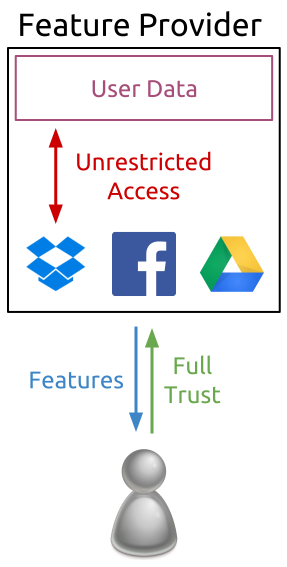
\includegraphics[height=2in]{./figs/out/TrustModel-Traditional.pdf}
    \caption{Traditional Trust Relationships}
    \label{fig:mitigation:trust:traditional}
  \end{subfigure}
  ~
  \begin{subfigure}[t]{0.48\textwidth}
    \centering
    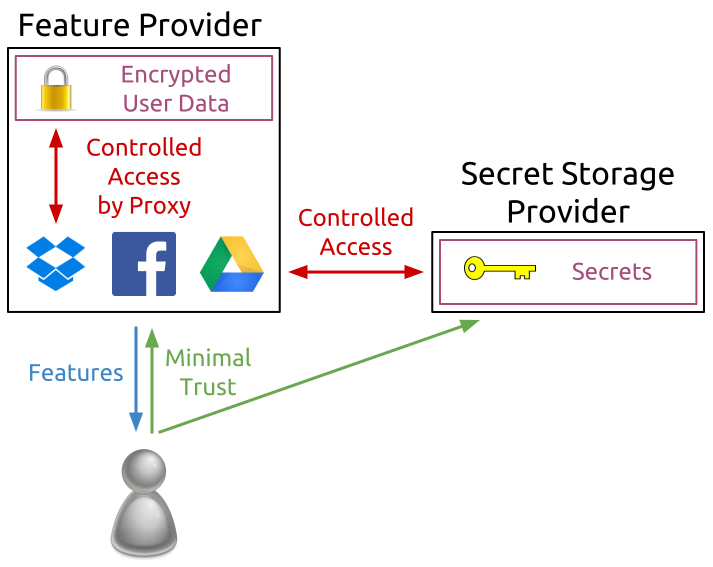
\includegraphics[height=2in]{./figs/out/TrustModel-Seperated.pdf}
    \caption{Distributed Trust Relationship}
    \label{fig:mitigation:trust:distributed}
  \end{subfigure}
  \caption{Trust Relationships}
  \label{fig:mitigation:trust}
\end{figure}

Techniques such as these are a from of ``trust distribution'' --
e.g. a technique for reducing trust in individual third parties by
instead spreading it across multiple parties
(Figure~\ref{fig:mitigation:trust}). Similar techniques have been used
within cryptographic protocols for the purpose of eliminating
single-points-of-trust~\cite{shamir1979}.\footnote{Such techniques
  also bear some resemble to previously proposed ``escrow systems,
  albeit with a somewhat opposite end-goal~\cite{denning1996}.}Such
techniques are capable of allowing users reduce or eliminate trust
surpluses across a range of use cases without introducing significant
additional usage burdens. While there are approaches to limiting third
party trust that aim to avoid trusting any third party (e.g. the OTR
chat protocol~\cite{otr-v3}), such techniques are often difficult to
apply generally or to use without imposing additional usability
burdens on end users. Trust distribution, however, provides a
relatively generic approach to to eliminating trust in any single
third party (or when coupled with techniques such
as~\cite{shamir1979}, even larger subsets of all involved parties).

To summarize, the basic practice of reducing the number of trusted
capabilities afforded to third parties is as follows: first, identity
any surplus trusted capabilities, next leverage cryptographic
techniques to limit third party access to these capabilities, finally,
leverage techniques such as SSaaS to store and control access to any
secret materials required by the aforementioned cryptographic
techniques in a manner that avoids burdening the end user with the
need to manage such secrets manually. This process eliminates trust
surplus and distributes user trust across multiple third parties in a
manner such that individual third parties can not subvert this
trust. As mentioned in \S~\ref{sec:analysis:violations}, such
arrangements do have the potential to encourage collusion-type trust
violations where multiple third parties work together to regain
capabilities that have bean denied to them. Mechanisms for
disincentivizing such violations will be discussed in the next
section.

\subsection{Disincentivizing Violations}


Distributed Trust Tor

Control Degree -> SSaaS, Etc
Disincentivize Violation -> Liability, Policy, Markets

%%  LocalWords:  SSaaS SSP OTR
